A decision tree is a classifier that makes several sequential decisions. The outcome of that sequence determines whether a data point belongs to one class or another. The structure of a decision tree \ref{fig:DT} is defined as a set of nodes ${x_1, ... , x_n}$ with edges ${e_1, .., e_{m}}$ between them. The edges are directed and there are no cycles in the network. The tree has one root $x_1$. With each data point we start at the root. The root node is fed information about a certain feature. Each node contains a rule that allows the node to make a decision. Each decision leads to a different node, where another decision is made. This process repeats itself until one of the leaf nodes is reached \cite{safavian1991survey}. From there we can determine what class our initial data point belonged to (either class $A$, $B$ or $C$ in the figure below. 
\begin{figure}[H]
    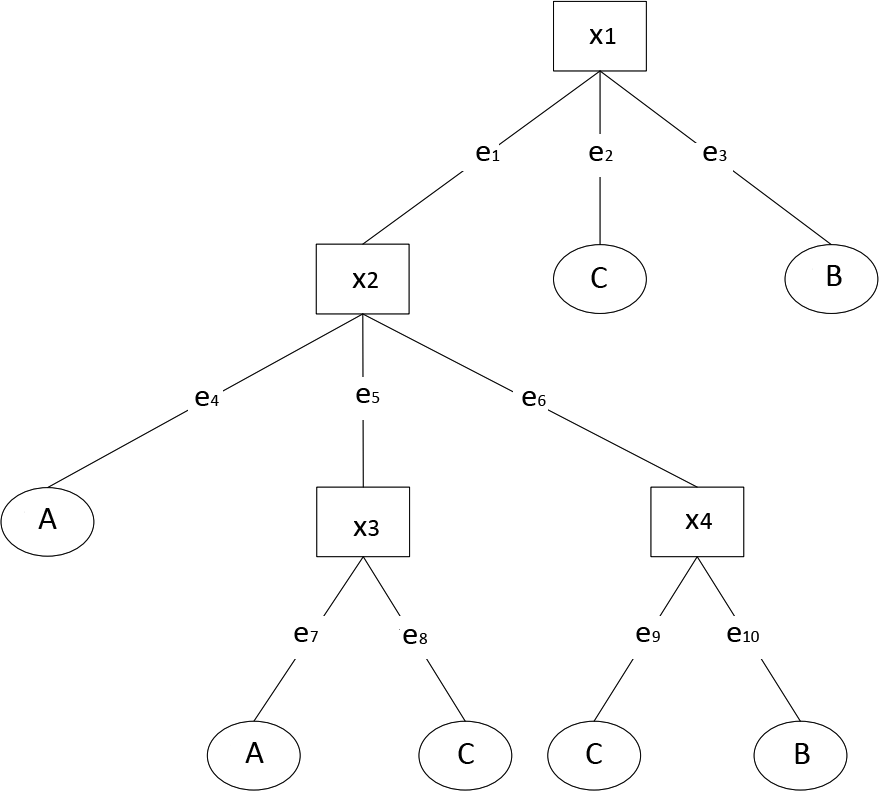
\includegraphics[width=80mm]{./img/decisiontree.png}
    \caption{Decision Tree example. $x_i$ are nodes where decisions are made. $e_j$ are edges leading down the tree to other nodes. $A,B,C$ are classes that instances are to be classified into.}
    \label{fig:DT}
\end{figure}

Decision trees are generally built or "grown" with a simple algorithm. Of course random selection of features is an option but this usually results in in low accuracy, because features that are irrelevant can be chosen as well. Another approach is to compare every feature and take the one with the best split. The best division is one that gains a lot of information about the data and their classes. For example: in classifying trees and plants, height might give more information about which class an instance belongs to than the colour of its leaves would. For each of the subsets that comes forth out of that division, the process is repeated until there is enough certainty that the remaining subset represents the class. This algorithm is also knowns as Fisher's Linear Discriminant Tree \cite{LópezChau20136283}. This does not take into account that a combination of features might make for an even better split, but it is a relatively efficient algorithm. A tree stops to grow when the impurity level is low enough. The impurity level is a metric to indicate what the chances are of misclassification. A simple example would be $impurity(node_j) = 1 - max(P(x_i = c_a) $. Here $x_i$ is the $i^{th}$ instance to be classified into class $c_a$. The opposite of growing a tree is called "pruning". This is done to increase the efficiency of the decision tree. Pruning is done by removing the least significant node(s).

In general, the more nodes a tree has, the more accurate it's classification will become. The downside is that the time to classify and train will increase the larger the tree becomes. It is impossible to optimize the accuracy and efficiency at the same time. The design of the tree is crucial, as each node splits up the dataset in a certain way. Dividing a datasets in the wrong order can make for significantly slower trees. Another problem is that errors may add up from node to node. If a node makes a wrong decision, there is no way for following nodes to compensate or correct. The advantage of the decision tree is it's computational efficiency, even with multivariate analyses \cite{safavian1991survey}, and its intuitive structure.